\let\negmedspace\undefined
\let\negthickspace\undefined
\documentclass[journal,12pt,onecolumn]{IEEEtran}
\usepackage{cite}
\usepackage{amsmath,amssymb,amsfonts,amsthm}
%\usepackage{algorithmic}
\usepackage{graphicx}
\usepackage{textcomp}
\usepackage{xcolor}
\usepackage{txfonts}
\usepackage{listings}
\usepackage{enumitem}
\usepackage{mathtools}
\usepackage{gensymb}
\usepackage[breaklinks=true]{hyperref}
\usepackage{tkz-euclide} % loads  TikZ and tkz-base
\usepackage{listings}
\usepackage{float}



\newtheorem{theorem}{Theorem}[section]
\newtheorem{problem}{Problem}
\newtheorem{proposition}{Proposition}[section]
\newtheorem{lemma}{Lemma}[section]
\newtheorem{corollary}[theorem]{Corollary}
\newtheorem{example}{Example}[section]
\newtheorem{definition}[problem]{Definition}
%\newtheorem{thm}{Theorem}[section] 
%\newtheorem{defn}[thm]{Definition}
%\newtheorem{algorithm}{Algorithm}[section]
%\newtheorem{cor}{Corollary}
\newcommand{\BEQA}{\begin{eqnarray}}
\newcommand{\EEQA}{\end{eqnarray}}
\newcommand{\define}{\stackrel{\triangle}{=}}
\theoremstyle{remark}
\newtheorem{rem}{Remark}
%\bibliographystyle{ieeetr}
\begin{document}
%
\providecommand{\pr}[1]{\ensuremath{\Pr\left(#1\right)}}
\providecommand{\prt}[2]{\ensuremath{p_{#1}^{\left(#2\right)} }}        % own macro for this question
\providecommand{\qfunc}[1]{\ensuremath{Q\left(#1\right)}}
\providecommand{\sbrak}[1]{\ensuremath{{}\left[#1\right]}}
\providecommand{\lsbrak}[1]{\ensuremath{{}\left[#1\right.}}
\providecommand{\rsbrak}[1]{\ensuremath{{}\left.#1\right]}}
\providecommand{\brak}[1]{\ensuremath{\left(#1\right)}}
\providecommand{\lbrak}[1]{\ensuremath{\left(#1\right.}}
\providecommand{\rbrak}[1]{\ensuremath{\left.#1\right)}}
\providecommand{\cbrak}[1]{\ensuremath{\left\{#1\right\}}}
\providecommand{\lcbrak}[1]{\ensuremath{\left\{#1\right.}}
\providecommand{\rcbrak}[1]{\ensuremath{\left.#1\right\}}}
\newcommand{\sgn}{\mathop{\mathrm{sgn}}}
\providecommand{\abs}[1]{\left\vert#1\right\vert}
\providecommand{\res}[1]{\Res\displaylimits_{#1}} 
\providecommand{\norm}[1]{\left\lVert#1\right\rVert}
%\providecommand{\norm}[1]{\lVert#1\rVert}
\providecommand{\mtx}[1]{\mathbf{#1}}
\providecommand{\mean}[1]{E\left[ #1 \right]}
\providecommand{\cond}[2]{#1\middle|#2}
\providecommand{\fourier}{\overset{\mathcal{F}}{ \rightleftharpoons}}
\newenvironment{amatrix}[1]{%
  \left(\begin{array}{@{}*{#1}{c}|c@{}}
}{%
  \end{array}\right)
}
%\providecommand{\hilbert}{\overset{\mathcal{H}}{ \rightleftharpoons}}
%\providecommand{\system}{\overset{\mathcal{H}}{ \longleftrightarrow}}
	%\newcommand{\solution}[2]{\textbf{Solution:}{#1}}
\newcommand{\solution}{\noindent \textbf{Solution: }}
\newcommand{\cosec}{\,\text{cosec}\,}
\providecommand{\dec}[2]{\ensuremath{\overset{#1}{\underset{#2}{\gtrless}}}}
\newcommand{\myvec}[1]{\ensuremath{\begin{pmatrix}#1\end{pmatrix}}}
\newcommand{\mydet}[1]{\ensuremath{\begin{vmatrix}#1\end{vmatrix}}}
\newcommand{\myaugvec}[2]{\ensuremath{\begin{amatrix}{#1}#2\end{amatrix}}}
\providecommand{\rank}{\text{rank}}
\providecommand{\pr}[1]{\ensuremath{\Pr\left(#1\right)}}
\providecommand{\qfunc}[1]{\ensuremath{Q\left(#1\right)}}
	\newcommand*{\permcomb}[4][0mu]{{{}^{#3}\mkern#1#2_{#4}}}
\newcommand*{\perm}[1][-3mu]{\permcomb[#1]{P}}
\newcommand*{\comb}[1][-1mu]{\permcomb[#1]{C}}
\providecommand{\qfunc}[1]{\ensuremath{Q\left(#1\right)}}
\providecommand{\gauss}[2]{\mathcal{N}\ensuremath{\left(#1,#2\right)}}
\providecommand{\diff}[2]{\ensuremath{\frac{d{#1}}{d{#2}}}}
\providecommand{\myceil}[1]{\left \lceil #1 \right \rceil }
\newcommand\figref{Fig.~\ref}
\newcommand\tabref{Table~\ref}
\newcommand{\sinc}{\,\text{sinc}\,}
\newcommand{\rect}{\,\text{rect}\,}
%%
%	%\newcommand{\solution}[2]{\textbf{Solution:}{#1}}
%\newcommand{\solution}{\noindent \textbf{Solution: }}
%\newcommand{\cosec}{\,\text{cosec}\,}
%\numberwithin{equation}{section}
%\numberwithin{equation}{subsection}
%\numberwithin{problem}{section}
%\numberwithin{definition}{section}
%\makeatletter
%\@addtoreset{figure}{problem}
%\makeatother

%\let\StandardTheFigure\thefigure
\let\vec\mathbf

\bibliographystyle{IEEEtran}





\bigskip

%\renewcommand{\thefigure}{\theenumi}
%\renewcommand{\thetable}{\theenumi}
%\renewcommand{\theequation}{\theenumi}

Q: If $a\left(\frac{1}{b} + \frac{1}{c}\right)$, $b\left(\frac{1}{c} + \frac{1}{a}\right)$, $c\left(\frac{1}{a} + \frac{1}{b}\right)$ are in arithmetic progression (AP), prove that $a$, $b$, $c$ are also in AP. \\


\solution
Common difference can be written as: 
\begin{align}
b\left(\frac{1}{c} + \frac{1}{a}\right) - a\left(\frac{1}{b} + \frac{1}{c}\right) &= c\left(\frac{1}{a} + \frac{1}{b}\right) - b\left(\frac{1}{c} + \frac{1}{a}\right) \nonumber \\
(b\left(\frac{1}{c} + \frac{1}{a}\right)+1) - (a\left(\frac{1}{b} + \frac{1}{c}\right)+1) &= (c\left(\frac{1}{a} + \frac{1}{b}\right)+1) - (b\left(\frac{1}{c} + \frac{1}{a}\right)+1) \nonumber \\ \implies
(b\left(\frac{1}{c} + \frac{1}{a}\right) + \frac{b}{b}) - (a\left(\frac{1}{b} + \frac{1}{c}\right) + \frac{a}{a}) &= (c\left(\frac{1}{a} + \frac{1}{b}\right) + \frac{c}{c}) - (b\left(\frac{1}{c} + \frac{1}{a}\right) + \frac{b}{b}) \nonumber \\ \implies
(b\left(\frac{1}{a} + \frac{1}{b} + \frac{1}{c}\right)) - (a\left(\frac{1}{a} + \frac{1}{b} + \frac{1}{c}\right)) &= (c\left(\frac{1}{a} + \frac{1}{b} + \frac{1}{c}\right)) - (b\left(\frac{1}{a} + \frac{1}{b} + \frac{1}{c}\right)) \nonumber \\ \implies
b - a &= c - b \nonumber 
\end{align}
Hence proved that $a$, $b$, $c$ are in AP. \\

%add table
\begin{table}[!h]

  \centering
  \begin{tabular}{|c|c|c|}
  \hline
    parameter & value & description \\
    \hline
    $x(0)$ & $a\left(\frac{1}{b} + \frac{1}{c}\right)$ & First Term of given AP \\
    \hline
    $d$ & ? & Common Difference of given AP \\
    \hline
    $x(n)$ & $(x(0) + nd)u(n)$ & General Term of given AP \\
    \hline
  \end{tabular}


\caption{Input Parameter Table}
\label{tab:11.9.5.16.tab1}
\end{table}

From table \ref{tab:11.9.5.16.tab1}
\begin{align}
X(z) &= x(0)\frac{1}{1- z^{-1}} + d\frac{z^{-1}}{(1-z^{-1})^2} \\
X(z) &= a\left(\frac{1}{b} + \frac{1}{c}\right)(\frac{1}{1- z^{-1}}) + (b - a)(\frac{1}{a} + \frac{1}{b} - \frac{1}{c})(\frac{z^{-1}}{(1-z^{-1})^2}) \quad \abs{z} > 1
\end{align}

\begin{figure}[h]
    \centering
    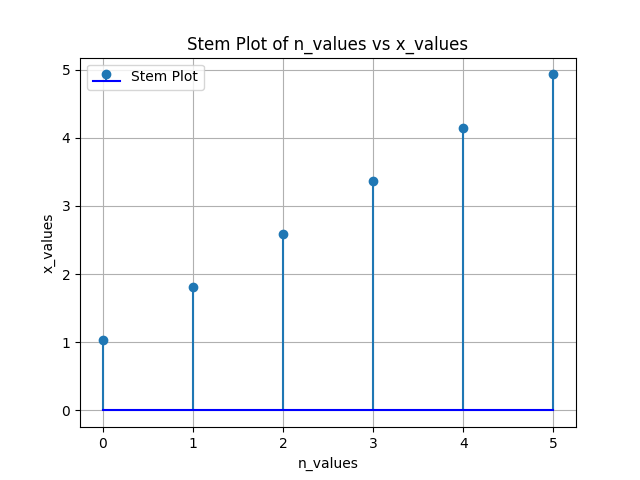
\includegraphics[width=\columnwidth]{./figs/fig1.png}
    \caption{graph with value of $a = 3, b = 5, c = 7$ }
\end{figure}


\end{document}
